\documentclass[a4paper,12pt]{article}
\usepackage[utf8]{inputenc}
\usepackage[T1]{fontenc}
\usepackage{textcomp}
\usepackage[english]{babel}
\usepackage{graphicx}
\usepackage{geometry}
\usepackage{titlesec}
\usepackage{array}
\usepackage{tabularx}
\usepackage{adjustbox}
\usepackage{multirow}
\usepackage[table,dvipsnames]{xcolor}
\makeatletter
\let\insert@pcolumn\insert@column
\makeatother
\usepackage{fancyhdr}
\usepackage{tcolorbox}
\tcbuselibrary{skins,breakable}
\usepackage{xurl}
\usepackage{setspace}
\usepackage{amsmath,amssymb}
\usepackage{subcaption}
\usepackage{float}
\usepackage{listings}
\usepackage{longtable}
\usepackage{booktabs}
\usepackage{enumitem}
\usepackage{tikz}
\usetikzlibrary{shapes,arrows,positioning,calc,fit,backgrounds,matrix,chains}
\usepackage{hyperref}

\hypersetup{
    colorlinks=true,
    linkcolor=NavyBlue,
    filecolor=magenta,      
    urlcolor=NavyBlue,
    citecolor=NavyBlue,
    pdfpagemode=FullScreen,
}

\geometry{top=2.5cm, bottom=2.5cm, left=2.5cm, right=2.5cm}
\setlength{\headheight}{15pt}
\setstretch{1.25}

% Official INPT Academic Color Palette
\definecolor{primary}{RGB}{0, 75, 160}
\definecolor{secondary}{RGB}{240, 245, 255}
\definecolor{tertiary}{RGB}{34, 139, 34}
\definecolor{accentorange}{RGB}{220, 100, 0}
\definecolor{tableheader}{RGB}{220, 235, 252}
\definecolor{riskred}{RGB}{255, 210, 210}
\definecolor{riskyellow}{RGB}{255, 250, 205}
\definecolor{riskgreen}{RGB}{220, 250, 220}
\definecolor{codegray}{RGB}{245, 245, 247}
\definecolor{codeborder}{RGB}{200, 205, 215}

% Section Titles Formatting
\titleformat{\section}{\normalfont\Large\bfseries\color{primary}}{\thesection}{1em}{}
\titleformat{\subsection}{\normalfont\large\bfseries\color{primary}}{\thesubsection}{1em}{}
\titleformat{\subsubsection}{\normalfont\normalsize\bfseries\color{primary}}{\thesubsubsection}{1em}{}

% Custom tcolorbox Environments
\newtcolorbox{calloutbox}[1][]{
    enhanced,
    colback=secondary,
    colframe=primary,
    arc=3mm,
    boxrule=1mm,
    fonttitle=\bfseries\color{white},
    coltitle=white,
    title=#1,
    left=4mm, right=4mm, top=3mm, bottom=3mm
}

\newtcolorbox{blockchainbox}[1][]{
    enhanced,
    colback=primary!5!white,
    colframe=primary,
    arc=2mm,
    boxrule=0.8mm,
    left=6mm, right=4mm, top=3mm, bottom=3mm,
    #1
}

\newtcolorbox{alertwarning}[1][]{
    enhanced,
    colback=riskred!30,
    colframe=accentorange!90!black,
    arc=2mm,
    boxrule=0.8mm,
    left=5mm, right=4mm, top=3mm, bottom=3mm,
    #1
}

% Code Listings Configuration
\lstdefinelanguage{json}{
    basicstyle=\ttfamily\footnotesize,
    showstringspaces=false,
    breaklines=true,
    frame=single,
    backgroundcolor=\color{codegray},
    rulecolor=\color{codeborder},
    stringstyle=\color{accentorange},
    commentstyle=\color{tertiary}\textit,
    morestring=[b]",
    morestring=[d]'
}

\lstdefinelanguage{golang}{
    keywords={package, import, func, return, if, else, var, const, type, struct, interface, range, for},
    keywordstyle=\color{primary}\bfseries,
    ndkeywords={string, int, int64, float64, bool, byte, error},
    ndkeywordstyle=\color{tertiary}\bfseries,
    identifierstyle=\color{black},
    sensitive=true,
    comment=[l]{//},
    morecomment=[s]{/*}{*/},
    commentstyle=\color{tertiary}\textit,
    stringstyle=\color{accentorange},
    morestring=[b]",
    morestring=[b]'
}

\lstdefinestyle{codeblock}{
    backgroundcolor=\color{codegray},
    basicstyle=\ttfamily\footnotesize,
    breaklines=true,
    frame=single,
    rulecolor=\color{codeborder},
    keywordstyle=\color{primary}\bfseries,
    commentstyle=\color{tertiary}\textit,
    stringstyle=\color{accentorange},
    numbers=left,
    numberstyle=\tiny\color{gray},
    numbersep=7pt,
    tabsize=2,
    showstringspaces=false
}
\lstset{style=codeblock}

% Headers and Footers
\pagestyle{fancy}
\fancyhf{}
\fancyhead[L]{\small \textcolor{primary}{\textbf{INPT -- BlockChain \& Smart Contract : ChainOps Cloud Platform}}}
\fancyhead[R]{\small \textcolor{gray}{Academic Year 2026/2027}}
\fancyfoot[L]{\small \textcolor{gray}{SESNUM (INE3) -- Bare-Metal Raspberry Pi Cluster}}
\fancyfoot[R]{\small \textbf{Page \thepage}}
\renewcommand{\headrulewidth}{0.6pt}
\renewcommand{\footrulewidth}{0.4pt}

\begin{document}

% ==============================================================================
% INSTITUTIONAL INPT COVER PAGE
% ==============================================================================
\begin{titlepage}
\centering

\begin{tcolorbox}[colframe=primary, colback=primary, width=\textwidth, boxrule=0mm, sharp corners, height=0.35cm]
\end{tcolorbox}

\vspace{0.25cm}


\includegraphics[width=0.22\textwidth]{inpt_logo.png}\\[0.25cm]

\begin{tcolorbox}[colframe=primary, colback=secondary, coltitle=primary, sharp corners=southwest, width=\textwidth, boxrule=1.2mm, top=0.45cm, bottom=0.45cm]
\centering
\vspace{0.15cm}
{\LARGE \textbf{\textcolor{primary}{ACADEMIC PROJECT REPORT}}}\\[0.35cm]
{\Large \textbf{ChainOps: Decentralized Cloud Infrastructure Engine}}\\[0.3cm]
{\large \textit{Immutable Orchestration, Smart Contracts, Smart Card HSM Custody, and Raft Quorum Consensus on a Physical 3-Node Raspberry Pi Cluster}}
\vspace{0.15cm}
\end{tcolorbox}

\vspace{0.35cm}

\begin{tcolorbox}[colframe=tertiary, colback=tertiary!10, width=0.94\textwidth, boxrule=0.6mm, sharp corners, left=0.6cm, right=0.6cm, top=0.3cm, bottom=0.3cm]
\centering
\textbf{\large Course Module: BlockChain \& Smart Contract}\\[0.15cm]
\textbf{\normalsize Academic Year 2026/2027}\\[0.25cm]
\textbf{\normalsize Authors / Project Contributors:}\\[0.15cm]
{\normalsize \textbf{\textcolor{primary}{ASLOUNE Yahya \qquad SALIOUI Ilyes \qquad SBAI Ahmed Taha}}}\\[0.3cm]
\textbf{\normalsize Under the Supervision of:}\\[0.15cm]
{\large \textbf{Prof. Meryeme AYACHE}}\\[0.1cm]
\textit{\small Professor at the National Institute of Posts and Telecommunications (INPT)}
\end{tcolorbox}

\vspace{0.35cm}

\begin{tcolorbox}[colframe=primary, colback=primary!10, sharp corners=northwest, width=0.90\textwidth, boxrule=0.8mm, top=0.25cm, bottom=0.25cm]
\centering
\textbf{\normalsize Department: Embedded Systems \& Digital Services (SESNUM -- INE3)}\\[0.1cm]
{\normalsize \textbf{National Institute of Posts and Telecommunications (INPT) -- Rabat, Morocco}}
\end{tcolorbox}

\vfill

{\small \textit{« Modern cloud computing infrastructure must no longer rely on blind trust in centralized root administrators, but on immutable cryptographic proofs, physical hardware security tokens, and fault-tolerant distributed consensus. »}}\\[0.35cm]

\begin{tcolorbox}[colframe=primary, colback=primary, width=\textwidth, boxrule=0mm, sharp corners, height=0.35cm]
\end{tcolorbox}

\end{titlepage}

\newpage
\pagenumbering{roman}
\tableofcontents
\newpage
\listoffigures
\listoftables
\newpage
\pagenumbering{arabic}

% ==============================================================================
% EXECUTIVE SUMMARY & ABSTRACT
% ==============================================================================
\section*{Executive Summary}
\addcontentsline{toc}{section}{Executive Summary}

Contemporary cloud orchestration infrastructures (typified by hyperscalers such as Amazon Web Services, Google Cloud Platform, and Microsoft Azure) are constructed around centralized trust perimeters. Core control-plane operations—including compute provisioning, memory quota enforcement, network ingress, and administrative access delegation—are recorded in conventional mutable relational databases or unchained key-value engines (e.g., standard Kubernetes \texttt{etcd}). In these models, a single compromised root credential or a rogue insider can tamper with cluster configurations, allocate unauthorized compute resources, or alter historical audit logs without triggering mathematical detection.

Developed as the capstone engineering project for the \textbf{BlockChain \& Smart Contract} course at INPT under the guidance of \textbf{Prof. Meryeme AYACHE}, this report introduces \textbf{ChainOps} : an enterprise-grade, decentralized cloud orchestration platform deployed across a physical bare-metal cluster of three \textbf{Raspberry Pi 4 (ARM64)} nodes. ChainOps revolutionizes cloud lifecycle management by treating every container provisioning request as an immutable financial transaction anchored into a 5-step cryptographic pipeline:

\begin{enumerate}[leftmargin=1.2cm]
    \item \textbf{Non-Custodial Cryptographic Client Signing}: Workloads are authorized exclusively via $secp256k1$ elliptic curve signatures, supporting both Web3 browser extensions (MetaMask) and physical \textbf{Smart Cards / Secure Hardware Modules} (Java Card tokens) executing on-chip APDU commands;
    \item \textbf{Deterministic Go Smart Contract Gatekeeper}: Enforces cluster-wide physical resource invariants via mathematical identity derivation (\texttt{ecrecover}) and hard limits to mathematically prevent Out-Of-Memory (OOM) host kernel panics;
    \item \textbf{Physical 3-Node Raft Consensus Engine}: Implements majority quorum ($N/2 + 1 = 2$ nodes) voting across physical Raspberry Pis with 150~ms heartbeats, leader election, and signed ballots to eliminate split-brain hazards;
    \item \textbf{Cryptographic Ledger via immudb}: Sequentially binds transactions into a SHA-256 Merkle tree state chain, exposing recalculable Merkle roots for real-time auditability and instantaneous tamper detection;
    \item \textbf{Physical Bare-Metal Kubernetes Orchestration}: Officially drives physical worker Pis via Kubernetes \texttt{client-go}, deploying pods with node affinity and automated self-healing runtimes to prevent \texttt{CrashLoopBackOff} on headless containers.
\end{enumerate}

To achieve true zero-trust networking without public IP addresses or local port forwarding, inter-node mTLS communication and client traffic are routed through Cloudflare Zero Trust Layer 4 TCP tunnel streams.

\vspace{0.4cm}
\noindent\rule{\textwidth}{0.4pt}
\vspace{0.2cm}

\section*{Résumé Analytique}
\addcontentsline{toc}{section}{Résumé Analytique}

Ce rapport présente \textbf{ChainOps}, une plateforme d'orchestration cloud décentralisée nativement intégrée sur un cluster physique bare-metal de 3 Raspberry Pi 4 (ARM64), réalisée dans le cadre du module \textbf{BlockChain \& Smart Contract} de l'INPT sous la supervision de \textbf{Mme Meryeme AYACHE}. L'architecture remplace la confiance implicite des infrastructures centralisées par un pipeline cryptographique déterministe articulé autour de cinq piliers : signature asymétrique cliente ($secp256k1$ et cartes à puce Java Card), validation par Smart Contract en Go avec respect strict des quotas mémoire physiques anti-OOM, consensus distribué Raft à majorité physique (quorum 2/3), persistance immuable dans immudb avec calcul de racines d'arbre de Merkle SHA-256, et ordonnancement physique bare-metal via Kubernetes \texttt{client-go}. L'isolation réseau est garantie par des tunnels Cloudflare Zero Trust Layer 4 TCP sans aucune exposition d'adresse IP locale.

\newpage

% ==============================================================================
% SECTION 1: INTRODUCTION, CONTEXT & PROBLEM STATEMENT
% ==============================================================================
\section{Introduction, Context \& Problem Statement}

\subsection{Technological Context: Vulnerabilities of Centralized Cloud Systems}

The containerization revolution led by Docker and Kubernetes has standardized software deployment globally. However, modern cluster management architectures retain an architectural flaw rooted in legacy client-server design: \textbf{centralized authority and blind database trust}.

In a standard Kubernetes deployment, the entire cluster configuration resides within \texttt{etcd}. Although \texttt{etcd} uses the Raft protocol to achieve fault tolerance across server replicas, it provides \textbf{zero cryptographic immutability guarantees}:
\begin{itemize}[leftmargin=1.2cm]
    \item An operating system user with root permissions on the master host can directly alter binary database keys, reconfiguring container privileges or injecting malicious pods without leaving a tamper-evident audit trail;
    \item Audit logging mechanisms rely on offloading plaintext JSON logs to external servers (Splunk, ElasticSearch, Datadog), which can be truncated, modified, or wiped by compromised administrative accounts;
    \item Traditional authentication mechanisms (X.509 client certificates, JWT Bearer tokens, static API keys) authenticate the channel, but do not cryptographically bind the author's identity to the exact binary payload of the deployed container.
\end{itemize}

\subsection{The Paradigm: Infrastructure as a Ledger}

To address these vulnerabilities, this project establishes the \textbf{Infrastructure-as-a-Ledger} paradigm.

\begin{calloutbox}[Core Axiom: Infrastructure as a Ledger]
In ChainOps, a cloud infrastructure operation (launching a container, allocating RAM, updating replica counts, or tearing down a service) is strictly defined as an \textbf{immutable state transaction}. It must be cryptographically signed by the operator's private key, deterministically validated against mathematical quota rules in a Smart Contract, agreed upon by a physical majority quorum through Raft consensus, committed to a Merkle-tree cryptographic ledger, and only then physically realized by the container runtime.
\end{calloutbox}

Table~\ref{tab:comparison_cloud} contrasts standard enterprise cloud platforms with the ChainOps DLT architecture.

\begin{table}[H]
\centering
\small
\resizebox{\linewidth}{!}{
\begin{tabular}{|l|p{6.5cm}|p{6.5cm}|}
\hline
\rowcolor{tableheader}
\textbf{Feature Dimension} & \textbf{Conventional Cloud (AWS / GCP / K8s)} & \textbf{ChainOps Architecture (Our Solution)} \\
\hline
\textbf{Identity \& Access} & Static API keys, session tokens, IAM roles & Asymmetric $secp256k1$ cryptographic signatures (EIP-191) \\
\hline
\textbf{Hardware Key Custody} & Software secrets, env vars, cloud KMS & Physical Smart Cards (Java Card) \& Secure Enclaves \\
\hline
\textbf{Admission Control} & Mutable webhook scripts (OPA / Gatekeeper) & Deterministic Go Smart Contract with hard hardware invariants \\
\hline
\textbf{Trust Topology} & Blind trust in centralized root admin & Distributed physical Raft quorum ($N/2 + 1$ physical Pis) \\
\hline
\textbf{State Persistence} & Mutable relational DB or unchained key-value & Append-only cryptographic ledger (\texttt{immudb}) \\
\hline
\textbf{Audit Verification} & Centralized, mutable log files & Mathematical SHA-256 Merkle root verification in sub-seconds \\
\hline
\textbf{Network Ingress} & Public IPs, open ports, NAT traversal & Cloudflare Zero Trust Layer 4 TCP tunnel with zero public IPs \\
\hline
\end{tabular}
}
\caption{Architectural comparison between conventional cloud infrastructure and ChainOps}
\label{tab:comparison_cloud}
\end{table}

\subsection{Academic Objectives \& Technical Specifications}

Within the scope of the \textbf{BlockChain \& Smart Contract} curriculum at INPT, our engineering team was tasked with designing, implementing, and validating an end-to-end bare-metal solution meeting the following specifications:
\begin{enumerate}[leftmargin=1.2cm]
    \item \textbf{Bare-Metal Physical Deployment}: Deploy on three physical Raspberry Pi 4 ARM64 single-board computers connected over a Gigabit Ethernet switch;
    \item \textbf{Strict Zero-Local-IP Dependency}: Enable worker Pis and external web clients to communicate with the master control plane entirely over a public domain managed by Cloudflare Zero Trust;
    \item \textbf{Physical Smart Card \& Web3 Key Custody}: Support non-custodial $secp256k1$ key custody using hardware tokens (Java Card tokens) and browser wallets (MetaMask);
    \item \textbf{Deterministic Smart Contract Gatekeeper}: Implement an automated resource controller in Go that performs elliptic curve recovery (\texttt{ecrecover}) and prevents cluster OOM crashes;
    \item \textbf{Distributed Raft Consensus Engine}: Build a 3-node physical Raft consensus cluster with heartbeats, election timeouts, and signed quorum voting ballots;
    \item \textbf{Cryptographic immudb Merkle Tree Ledger}: Persist all state transitions into SHA-256 hash chains with real-time Merkle root generation and automated tamper detection;
    \item \textbf{Production Kubernetes Orchestration}: Translate approved ledger transactions into native Kubernetes objects via official \texttt{client-go} drivers.
\end{enumerate}

\newpage

% ==============================================================================
% SECTION 2: PHYSICAL CLUSTER HARDWARE & ZERO-TRUST TOPOLOGY
% ==============================================================================
\section{Physical Cluster Hardware \& Zero-Trust Network Topology}

\subsection{Physical Bare-Metal Raspberry Pi 4 Cluster}

The platform executes on a dedicated 3-node physical Raspberry Pi 4 bare-metal cluster. Operating directly on bare metal exposes the software stack to realistic physical constraints: hardware CPU throttling, limited physical RAM, and kernel cgroup accounting.

\begin{table}[H]
\centering
\small
\resizebox{\linewidth}{!}{
\begin{tabular}{|l|l|l|l|p{4.5cm}|}
\hline
\rowcolor{tableheader}
\textbf{Node Identifier} & \textbf{Cluster Role} & \textbf{Architecture} & \textbf{Local LAN IP} & \textbf{Hardware Specifications} \\
\hline
\textbf{pi-node-01} & Master (Raft Leader) & ARM64 (BCM2711) & 192.168.1.212 & 4 Cores @ 1.5 GHz, 3,794 MB RAM, Debian 11 \\
\hline
\textbf{pi-worker-1-afe458a1} & Worker 1 (Raft Follower) & ARM64 (BCM2711) & 192.168.1.213 & 4 Cores @ 1.5 GHz, 3,794 MB RAM, Debian 11 \\
\hline
\textbf{pi-worker-2-d50675de} & Worker 2 (Raft Follower) & ARM64 (BCM2711) & 192.168.1.214 & 4 Cores @ 1.5 GHz, 3,794 MB RAM, Debian 11 \\
\hline
\rowcolor{secondary}
\textbf{Total Cluster Pool} & \textbf{High-Availability} & \textbf{ARM64 (12 Cores)} & \textbf{Zero Public IPs} & \textbf{11,382 MB Total Physical RAM} \\
\hline
\end{tabular}
}
\caption{Physical bare-metal hardware specifications of the Raspberry Pi cluster}
\label{tab:hardware_specs}
\end{table}

\subsection{End-to-End System Topology}

The physical deployment connects three tiers of infrastructure without requiring public IPv4 addresses, static port forwarding, or centralized VPN concentrators:
\begin{itemize}[leftmargin=1.2cm]
    \item \textbf{Client Layer (Web3 \& Key Custody)}: Web browsers running MetaMask or localized cryptographic keypairs initiate JSON-RPC deployment payloads, signing each request via non-custodial $secp256k1$ elliptic curve cryptography;
    \item \textbf{Edge Layer (Cloudflare Zero Trust)}: Terminates external HTTPS traffic on \url{https://bc.aslouneyahya.com} and reverse-proxies requests through an encrypted \texttt{cloudflared} tunnel to port 8080 on the master node. In parallel, it provisions a raw Layer~4 TCP stream for \url{k3s.aslouneyahya.com} targeting port 6443;
    \item \textbf{Master Node (\texttt{pi-node-01}, 192.168.1.212)}: Runs the ChainOps Go daemon (port 8080), the immudb immutable ledger service (port 3322), and the K3s control plane server (port 6443);
    \item \textbf{Physical Worker Nodes (\texttt{pi-worker-1-afe458a1} \& \texttt{pi-worker-2-d50675de})}: Connect to the K3s server via local \texttt{cloudflared access tcp} client bridges, executing application pods on bare-metal ARM64 \texttt{containerd} runtimes.
\end{itemize}

\subsection{Solving the Kubernetes Control Plane Ingress: Layer 4 TCP Tunneling}

A core engineering hurdle involved connecting distributed worker Pis to the control plane over the public internet without port forwarding.

\begin{alertwarning}
\textbf{Root Cause Analysis: Layer 7 HTTPS Proxy Failure:}
Initially, \texttt{k3s.aslouneyahya.com} was configured as an HTTP/HTTPS reverse proxy hostname in Cloudflare. This caused a catastrophic failure loop on worker nodes:
\begin{lstlisting}
Failed to connect to https://127.0.0.1:6444/cacerts: 403 Forbidden
\end{lstlisting}
\textbf{Diagnosis:} Layer 7 reverse proxies terminate TLS at Cloudflare's edge. However, Kubernetes internode clustering relies on \textbf{Mutual TLS (mTLS)} where both client and server present X.509 certificates. By terminating TLS and rewriting the HTTP \texttt{Host} header to \texttt{127.0.0.1:6444}, Cloudflare stripped client certificates, causing K3s server to instantly reject the handshake with HTTP 403.
\end{alertwarning}

\begin{calloutbox}[Production Solution: Layer 4 Raw TCP Tunnel Stream]
To preserve end-to-end mTLS without exposing physical public IP addresses, we re-architected the tunnel:
\begin{itemize}
    \item Cloudflare Edge Rule: Route \texttt{k3s.aslouneyahya.com} as raw \textbf{TCP to 127.0.0.1:6443};
    \item Worker nodes run a local client bridge daemon (\texttt{k3s-tcp-tunnel.service}):
    \begin{lstlisting}[language=bash]
cloudflared access tcp --hostname k3s.aslouneyahya.com --url 127.0.0.1:6443
    \end{lstlisting}
    \item The local K3s agent points to \texttt{https://127.0.0.1:6443}. Raw TCP packets stream across Cloudflare untouched, allowing native Kubernetes mTLS to negotiate cleanly without local network dependencies.
\end{itemize}
\end{calloutbox}



\newpage

% ==============================================================================
% SECTION 3: CRYPTOGRAPHIC IDENTITY & SMART CARD HSM CUSTODY
% ==============================================================================
\section{Cryptographic Identity, Smart Cards \& Hardware Key Custody}

\subsection{Mathematical Foundations: $secp256k1$ Elliptic Curve Cryptography}

ChainOps operates entirely without usernames, passwords, or centralized database credentials. Identity is derived directly from asymmetric key cryptography on the Koblitz elliptic curve $secp256k1$, defined over the finite field $\mathbb{F}_p$ by the Weierstrass equation:
\begin{equation}
y^2 = x^3 + 7 \pmod p
\end{equation}
where $p = 2^{256} - 2^{32} - 977$.

An operator generates a private key $k \in [1, n-1]$ and derives the corresponding public key point $K = k \cdot G$, where $G$ is the uncompressed base generator point. The Ethereum-compatible address is computed as the last 20 bytes of the Keccak-256 hash of the uncompressed public key coordinates:
\begin{equation}
\text{Address} = \text{Keccak256}(K_x \,\|\, K_y)[12..31]
\end{equation}

When an operator prepares a deployment request, the canonical JSON payload is prefixed according to Ethereum Improvement Proposal \textbf{EIP-191}:
\begin{equation}
m = \text{Keccak256}\Big(\text{"\textbackslash x19Ethereum Signed Message:\textbackslash n"} + \text{len}(\text{Payload}) + \text{Payload}\Big)
\end{equation}
The resulting signature tuple $\sigma = (r, s, v)$ allows deterministic recovery of $K$ via elliptic curve point arithmetic.

\subsection{Smart Card Architecture \& Hardware Key Isolation (Java Card)}

While browser extensions (such as MetaMask) provide convenient key storage for desktop developers, enterprise operational security requires \textbf{Hardware Security Module (HSM)} and Secure Element isolation to protect high-privilege infrastructure keys from host operating system compromise, memory scraping, and zero-day keyloggers.

\begin{calloutbox}[Smart Card Hardware Security Boundary (Java Card)]
To anchor cryptographic identity into hardware, ChainOps supports physical \textbf{Java Card} smart cards (compliant with the Java Card 3.0 specification). In this model, the private key $k$ is generated on-chip inside the card's tamper-resistant Secure Element (SE) and \textbf{can never be exported or read over the I/O bus}.
\end{calloutbox}

The cryptographic signing exchange operates via a strict ISO/IEC 7816-4 challenge-response protocol:
\begin{enumerate}[leftmargin=1.2cm]
    \item The client workstation computes the 32-byte Keccak-256 hash digest $m$ of the canonical deployment JSON payload;
    \item The client workstation transmits an ISO/IEC 7816-4 APDU command to the smart card reader over the standard CCID interface;
    \item The card verifies the operator's physical PIN against securely stored on-chip credentials;
    \item The card's internal cryptographic coprocessor performs on-chip scalar multiplication $k \cdot G$ to compute the signature components $r = R_x \pmod n$ and $s = k^{-1}(m + r k) \pmod n$;
    \item The card outputs the 65-byte signature tuple $\sigma = (r, s, v)$ accompanied by the success status word \texttt{0x90 0x00}. Even in the event of a full operating system or kernel compromise on the operator's workstation, the private key remains physically isolated and non-extractable.
\end{enumerate}

\newpage

% ==============================================================================
% SECTION 4: THE GO SMART CONTRACT GATEKEEPER ENGINE
% ==============================================================================
\section{The Go Smart Contract Gatekeeper Engine}

\subsection{Deterministic Rule Enforcement (\texttt{pkg/contract})}

Upon receiving a deployment transaction on \texttt{POST /api/deployments}, the Go daemon executes the \textbf{Smart Contract Gatekeeper} (\texttt{pkg/contract/gatekeeper.go}). Unlike user-space admission controllers that execute arbitrary scripts, the Smart Contract Gatekeeper enforces deterministic constraints derived from physical bare-metal capacity:

\begin{enumerate}[leftmargin=1.2cm]
    \item \textbf{Mathematical Cryptographic Identity Verification}:
    The Gatekeeper reconstructs the EIP-191 message prefix and recovers the signer's public key using elliptic curve point arithmetic:
    \begin{lstlisting}[language=golang]
pubKey, err := crypto.SigToPub(messageHash, signatureBytes)
if err != nil {
    return nil, fmt.Errorf("cryptographic verification failed: %w", err)
}
recoveredAddress := crypto.PubkeyToAddress(*pubKey).Hex()
    \end{lstlisting}
    If the recovered address fails to match the transaction's \texttt{signerAddress}, the request is rejected with HTTP 401.
    \item \textbf{Cluster Memory Conservation Invariant}:
    To prevent physical out-of-memory kernel panics on ARM64 nodes, the contract enforces:
    \begin{equation}
    \sum_{i=1}^{M} \text{AllocatedRAM}_i + \text{RequestedRAM} \le 11,382 \text{ MB}
    \end{equation}
    where 11,382~MB represents the total calibrated memory pool across all three Raspberry Pis.
    \item \textbf{Workload Container Size Caps}:
    Individual containers are capped at 2,048~MB of RAM and 2 physical CPU cores to guarantee that a single pod cannot monopolize an entire worker Pi.
    \item \textbf{DNS-1123 RFC Validation}:
    Validates that the workload name matches the regex \lstinline|^[a-z0-9]([-a-z0-9]*[a-z0-9])?$|, preventing manifest injection attacks into Kubernetes.
\end{enumerate}



\newpage

% ==============================================================================
% SECTION 5: DISTRIBUTED RAFT CONSENSUS PROTOCOL
% ==============================================================================
\section{Distributed Raft Consensus on Physical Raspberry Pis}

\subsection{Formal Raft State Machine Replication (\texttt{pkg/consensus})}

In centralized cloud architectures, a single compromised server can unilaterally modify cluster state. ChainOps prevents unilateral action by embedding a distributed \textbf{Raft consensus engine} across the physical Raspberry Pis.

Raft decomposes distributed consensus into three orthogonal subproblems:
\begin{enumerate}[leftmargin=1.2cm]
    \item \textbf{Leader Election}: At any time, exactly one node acts as Leader (\texttt{pi-node-01}), while all other nodes operate as Followers (\texttt{pi-worker-1-\allowbreak afe458a1}, \texttt{pi-worker-2-\allowbreak d50675de});
    \item \textbf{Heartbeat \& Term Synchronization}: The Leader broadcasts periodic heartbeat messages every 150~ms to maintain its authority. If a Follower detects no heartbeat within a randomized election timeout window (300~ms to 500~ms), it increments its term counter, transitions to Candidate, and broadcasts a \texttt{RequestVote} RPC;
    \item \textbf{Log Replication \& Quorum Agreement}: Before committing a transaction, the Leader broadcasts a proposal hash to all Followers. Each physical Pi verifies local state invariants and replies with a signed cryptographic ballot.
\end{enumerate}

\begin{table}[H]
\centering
\small
\resizebox{\linewidth}{!}{
\begin{tabular}{|l|l|p{8.5cm}|}
\hline
\rowcolor{tableheader}
\textbf{Raft Protocol Parameter} & \textbf{Production Value} & \textbf{Physical Justification on Raspberry Pi Cluster} \\
\hline
\textbf{Active Leader} & \texttt{pi-node-01} & Control plane host running K3s server and immudb daemon \\
\hline
\textbf{Majority Quorum Threshold} & $\lfloor N/2 \rfloor + 1 = 2$ nodes & Minimum positive votes required to commit without split-brain risk \\
\hline
\textbf{Heartbeat Interval} & 150 ms & Sub-second detection of physical node disconnects or power losses \\
\hline
\textbf{Election Timeout Window} & 300 ms -- 500 ms & Randomized jitter prevents split votes during simultaneous candidate elections \\
\hline
\end{tabular}
}
\caption{Calibrated operational parameters of the physical Raft consensus protocol}
\label{tab:raft_params}
\end{table}

\subsection{Fault Tolerance \& Network Partition Scenarios}

The physical 3-node Raft consensus engine deterministically handles three operational scenarios:
\begin{enumerate}[leftmargin=1.2cm]
    \item \textbf{Scenario A: Nominal 3/3 Consensus}: All three physical Raspberry Pis are operational and communicate across the Gigabit Ethernet switch. The leader receives positive ballots from both followers, reaching 100\% consensus ($3/3$). The transaction is committed and logged to immudb;
    \item \textbf{Scenario B: Single-Node Hardware Failure (2/3 Quorum)}: If one physical worker suffers a sudden power loss or hardware failure, the leader continues to receive a valid ballot from the remaining worker. Because $2 \ge \lfloor 3/2 \rfloor + 1 = 2$, majority quorum is preserved, allowing zero-downtime workload deployments;
    \item \textbf{Scenario C: Network Partition \& Split-Brain Mitigation (1/3)}: If an isolated leader loses connectivity to both physical workers, it collects only its own vote ($1/3$). Failing the majority threshold, the proposal is rejected, preventing inconsistent split-brain writes across partitioned segments.
\end{enumerate}

When a majority quorum is assembled, the leader creates a signed \texttt{ConsensusReceipt}:
\begin{lstlisting}[language=golang]
type ConsensusReceipt struct {
    Term          int64           `json:"term"`
    LeaderNode    string          `json:"leaderNode"`
    TotalNodes    int             `json:"totalNodes"`
    PositiveVotes int             `json:"positiveVotes"`
    QuorumReached bool            `json:"quorumReached"`
    Votes         []ConsensusVote `json:"votes"`
}
\end{lstlisting}
This receipt constitutes non-repudiable mathematical evidence of distributed agreement before state commitment.

\newpage

% ==============================================================================
% SECTION 6: IMMUTABLE LEDGER VIA IMMUDB & MERKLE TREES
% ==============================================================================
\section{Immutable Ledger Storage via immudb \& Merkle Trees}

\subsection{Cryptographic Hash Chaining}

Every approved transaction is committed to \textbf{immudb} (\texttt{pkg/ledger/immudb.go}). The cryptographic foundation is recursive SHA-256 state chaining:
\begin{equation}
H_0 = \text{0x0000000000000000000000000000000000000000000000000000000000000000}
\end{equation}
\begin{equation}
H_n = \text{SHA256}(H_{n-1} \,\|\, \text{TxID}_n \,\|\, \text{Timestamp}_n \,\|\, \text{SignerAddress}_n \,\|\, \text{PayloadHash}_n)
\end{equation}

Transactions in immudb form a dual-layer cryptographic structure:
\begin{enumerate}[leftmargin=1.2cm]
    \item \textbf{Sequential Hash Chain}: Each state block links recursively to its immediate predecessor via $H_n = \text{SHA256}(H_{n-1} \,|\,\, \text{TxID}_n \,|\,\, \dots)$, ensuring total temporal ordering;
    \item \textbf{Binary Merkle Tree}: Transactions simultaneously populate the leaves of a balanced binary Merkle tree. Pairwise hashes are recursively computed upward until deriving the cluster's active Merkle Root (e.g., \texttt{0xedb3e527...4d01d0}). This architecture enables logarithmic $O(\log N)$ inclusion proofs for third-party client verification.
\end{enumerate}

\subsection{Real-Time Audit Verification \& Tamper Detection Workflow}

The endpoint \texttt{GET /api/ledger/audit} allows third-party observers to cryptographically verify cluster history from Genesis without administrative credentials. The audit algorithm sequentially traverses each committed transaction from block $k=1$ to tip $N$, re-evaluating $H_k = \text{SHA256}(H_{k-1} \,|\,\, \dots)$ and asserting equality with the stored record. Once all individual block hashes match, the overall Merkle tree is reconstructed to confirm that the recalculated root matches the immudb root header.

To prove tamper resistance in demonstrations, calling \lstinline|POST /api/ledger/simulate-tamper| alters an on-disk record. The audit algorithm immediately flags the fraud:
\begin{lstlisting}[language=json]
{
  "valid": false,
  "brokenTxId": 2,
  "reason": "Tamper detected: stored block hash does not match recalculated hash"
}
\end{lstlisting}

\newpage

% ==============================================================================
% SECTION 7: KUBERNETES ORCHESTRATION & STATE SYNCHRONIZATION
% ==============================================================================
\section{Physical Kubernetes Orchestration via client-go}

\subsection{Manifest Synthesis \& Node Affinity Scheduling}

Upon confirmed ledger commitment, the orchestrator (\texttt{pkg/k3s/orchestrator.go}) translates the transaction into Kubernetes resources using official \texttt{client-go} drivers:
\begin{itemize}[leftmargin=1.2cm]
    \item \textbf{Deployment Synthesis}: Dynamically provisions an \texttt{apps/v1 Deployment} and \texttt{v1 Service};
    \item \textbf{Physical Worker Node Affinity}: To protect the Master Pi from compute overload, the orchestrator injects a strict \texttt{nodeAffinity} targeting worker hostnames:
    \begin{lstlisting}[language=golang]
Affinity: &corev1.Affinity{
    NodeAffinity: &corev1.NodeAffinity{
        RequiredDuringSchedulingIgnoredDuringExecution: &corev1.NodeSelector{
            NodeSelectorTerms: []corev1.NodeSelectorTerm{
                {
                    MatchExpressions: []corev1.NodeSelectorRequirement{
                        {
                            Key:      "kubernetes.io/hostname",
                            Operator: corev1.NodeSelectorOpIn,
                            Values:   []string{"pi-worker-1-afe458a1", "pi-worker-2-d50675de"},
                        },
                    },
                },
            },
        },
    },
}
    \end{lstlisting}
    \item \textbf{Automated Entrypoint Injection (Anti-CrashLoopBackOff)}:
    Headless containers (e.g., \texttt{python:3.11-alpine}) terminate immediately with exit code 0 when started without an interactive TTY. ChainOps automatically detects runtime images and injects a non-blocking background server:
    \begin{lstlisting}[language=golang]
if strings.Contains(image, "python") {
    container.Command = []string{"sh", "-c", "python3 -m http.server " + portStr}
}
    \end{lstlisting}
\end{itemize}

Workload execution follows a strict finite state progression across seven distinct phases:
\begin{enumerate}[leftmargin=1.2cm]
    \item \textbf{Form Configuration}: The operator defines container parameters (image, replicas, port, memory quota) in the web console;
    \item \textbf{Cryptographic Signing}: The client workstation computes the EIP-191 digest and signs the canonical payload via MetaMask or local keypair;
    \item \textbf{Smart Contract Evaluation}: The Go Gatekeeper validates signature authenticity, DNS-1123 compliance, and cluster RAM caps;
    \item \textbf{Distributed Raft Quorum}: The leader broadcasts the proposal and collects majority signed ballots ($2/3$ or $3/3$);
    \item \textbf{Immutable Ledger Persistence}: The approved transaction is written to immudb with its updated Merkle root;
    \item \textbf{client-go Manifest Scheduling}: The orchestrator synthesizes the Kubernetes Deployment and applies node affinity constraints;
    \item \textbf{Active Pod Execution}: The pod transitions to \texttt{Running 1/1 Ready} on a physical worker Pi.
\end{enumerate}

\subsection{Internal Go Package Architecture}

The Go cluster daemon codebase (\texttt{cluster-daemon/pkg/}) is structured into six decoupled packages:
\begin{itemize}[leftmargin=1.2cm]
    \item \texttt{pkg/api}: Implements the HTTP REST API gateway, routing client traffic to internal handlers;
    \item \texttt{pkg/crypto}: Encapsulates elliptic curve cryptography, executing Keccak-256 hashing and \texttt{ecrecover};
    \item \texttt{pkg/contract}: Hosts the deterministic Smart Contract Gatekeeper enforcing hardware memory and CPU invariants;
    \item \texttt{pkg/consensus}: Implements the physical 3-node Raft consensus engine, term tracking, and signed ballots;
    \item \texttt{pkg/ledger}: Encapsulates the immudb client driver, linear hash chaining, and real-time Merkle tree audits;
    \item \texttt{pkg/k3s}: Interfaces with the Kubernetes control plane via official \texttt{client-go} drivers for manifest synthesis.
\end{itemize}

The platform's data model links client intent, consensus proofs, and physical infrastructure across four core entities:
\begin{itemize}[leftmargin=1.2cm]
    \item \textbf{Signed Request}: Client payload containing \texttt{signerAddress}, signature $\sigma = (r, s, v)$, canonical JSON body, and timestamp;
    \item \textbf{Consensus Receipt}: Raft quorum ballot proof containing the election term, leader ID, positive vote count, and quorum state;
    \item \textbf{Ledger Transaction}: The immutable record stored in immudb with monotonic \texttt{txId}, \texttt{blockHash}, \texttt{previousHash}, active \texttt{merkleRoot}, and embedded consensus receipt;
    \item \textbf{K3s Workload Status}: The active cluster state managed by \texttt{client-go}, including \texttt{deploymentId}, assigned physical host (\texttt{pi-worker-1}), internal IP, and pod execution phase.
\end{itemize}

\newpage

% ==============================================================================
% SECTION 8: EXPERIMENTAL RESULTS & VISUAL PRODUCTION TOUR
% ==============================================================================
\section{Experimental Evaluation \& Visual Production Tour}

All experiments were executed on the live bare-metal cluster in production. This section analyzes the 10 production views validating full operational readiness.

\subsection{Web3 Authentication Portal}

Figure~\ref{fig:bc_login} presents the decentralized authentication portal hosted at \url{https://bc.aslouneyahya.com}.

\begin{figure}[H]
\centering
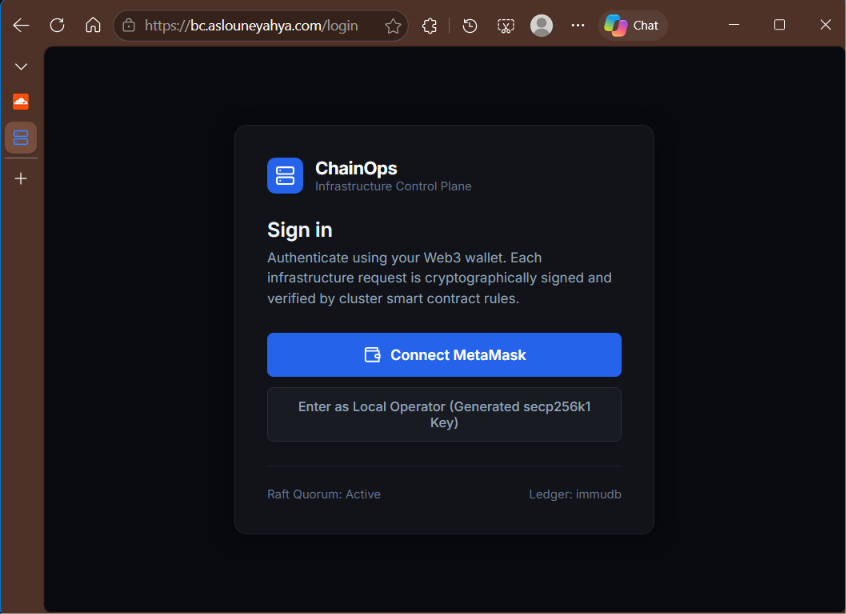
\includegraphics[width=0.82\linewidth]{figures/bc_login.png}
\caption{Decentralized Web3 authentication supporting MetaMask and Local Operator Keypairs}
\label{fig:bc_login}
\end{figure}

Operators choose between browser extensions (MetaMask) or zero-dependency in-memory $secp256k1$ keypairs signing in under 1~ms.

\subsection{5-Step Consensus Deployment Modal}

Figure~\ref{fig:new_deployment_steps} displays the interactive modal visualizing each stage of the cryptographic consensus pipeline in real time.

\begin{figure}[H]
\centering
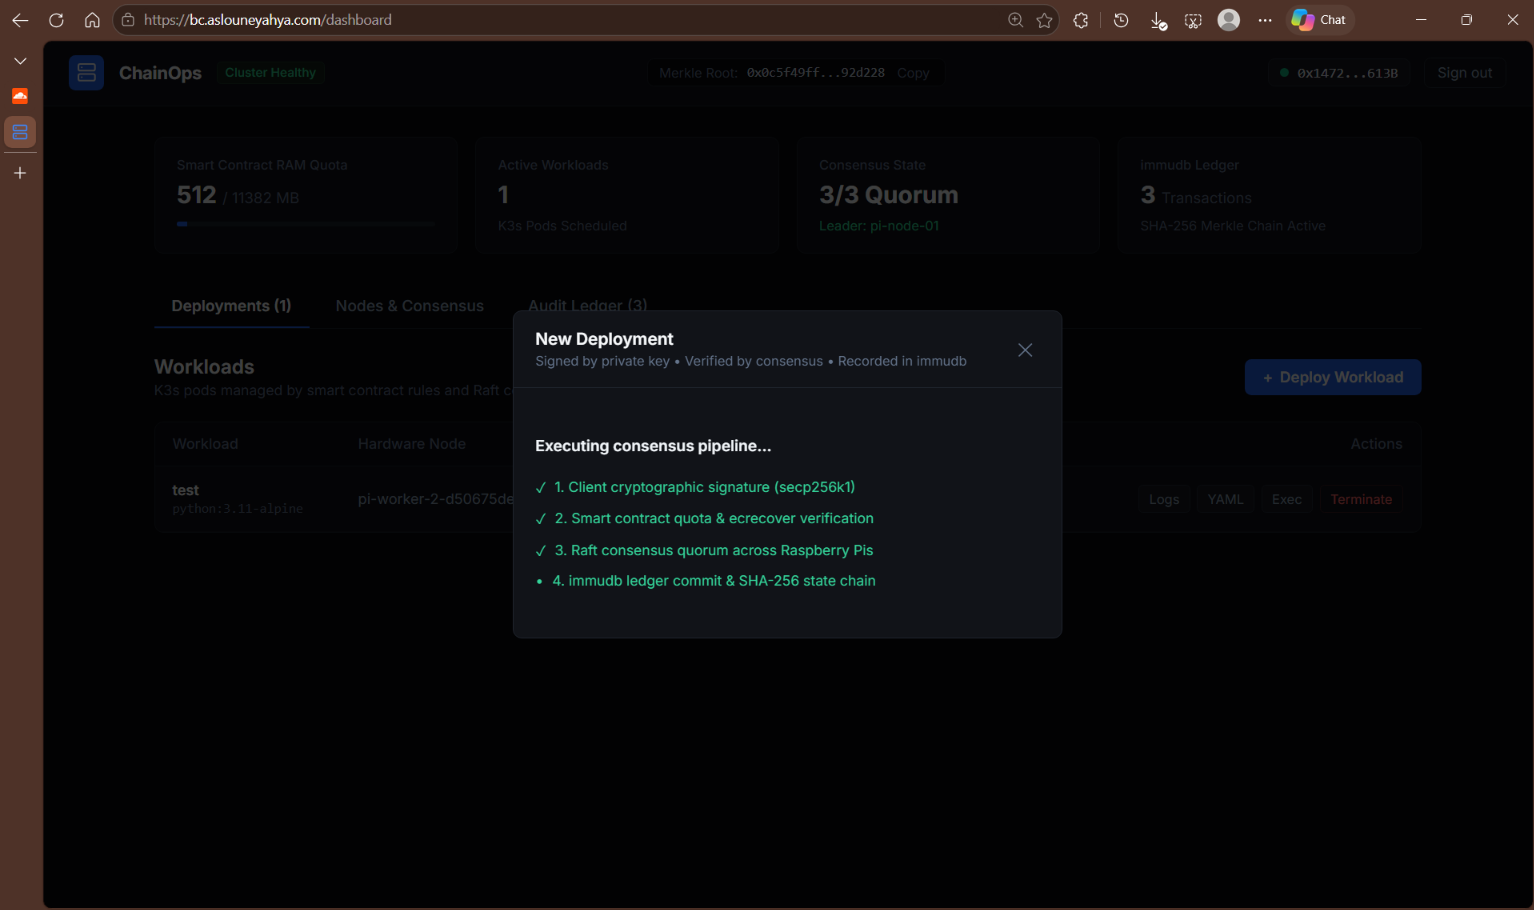
\includegraphics[width=0.82\linewidth]{figures/new_deployment_steps.png}
\caption{Live modal tracking client signing, smart contract validation, Raft consensus, and immudb commit}
\label{fig:new_deployment_steps}
\end{figure}

\subsection{Live Pod Execution on Physical Worker Node}

Figure~\ref{fig:test2_running} confirms container \texttt{test2} (\texttt{python:3.11-alpine}) executing in state \texttt{Running (1/1 Ready)} on node \texttt{pi-worker-1-\allowbreak afe458a1} with internal pod IP \texttt{10.42.4.2}.

\begin{figure}[H]
\centering
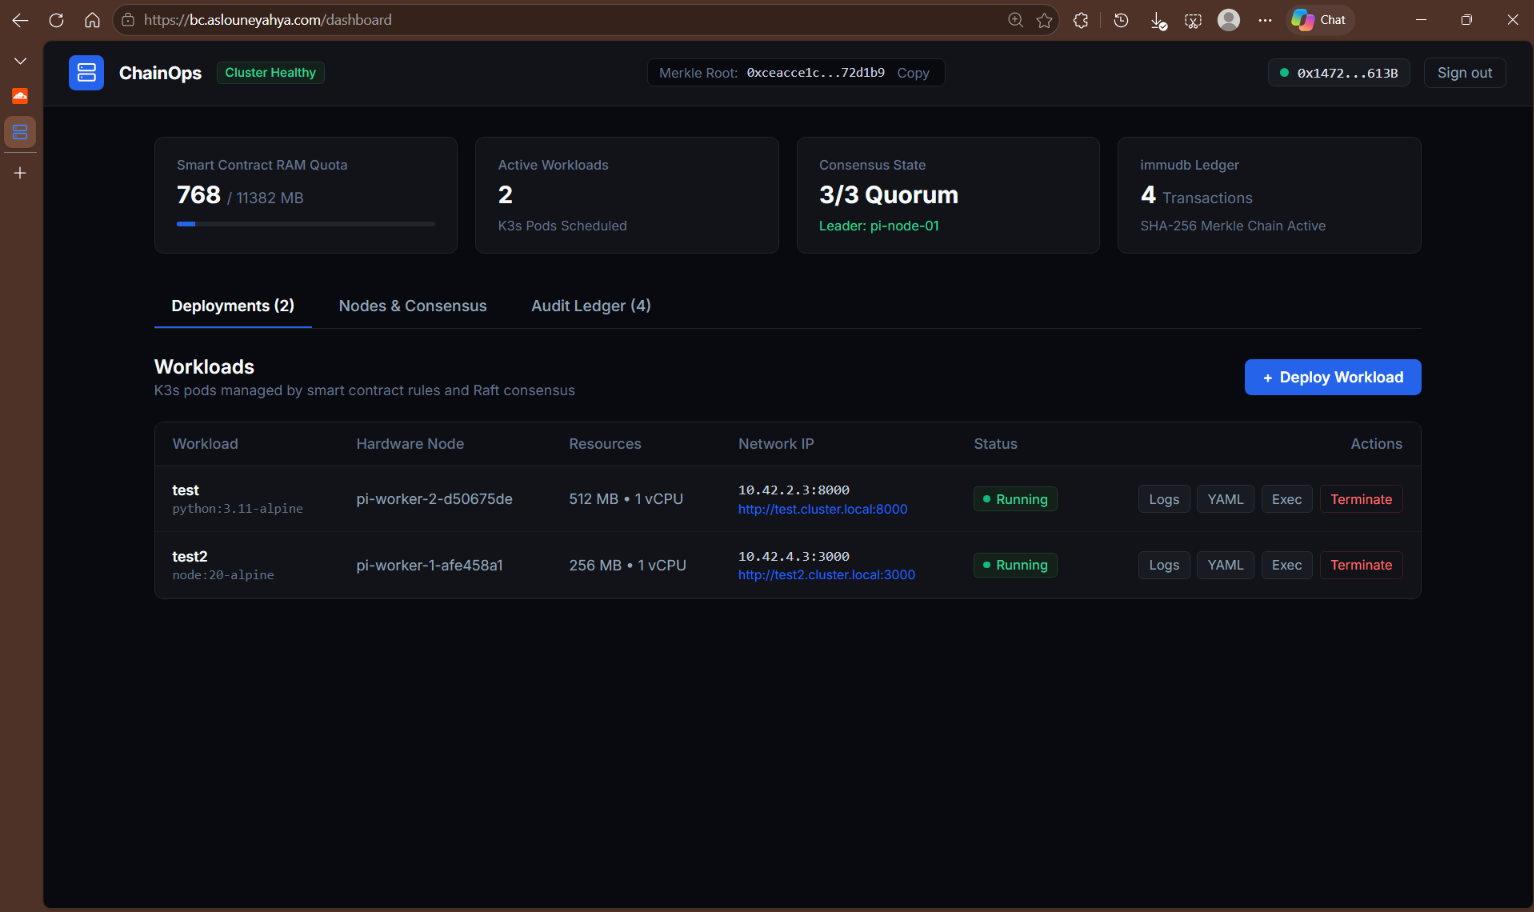
\includegraphics[width=0.82\linewidth]{figures/test2_running.png}
\caption{Production container \texttt{test2} scheduled and executing on physical worker node}
\label{fig:test2_running}
\end{figure}

Figure~\ref{fig:test2_deployment} displays the manifest drawer, showing the dynamic YAML synthesized by \texttt{client-go} and live streaming execution logs.

\begin{figure}[H]
\centering
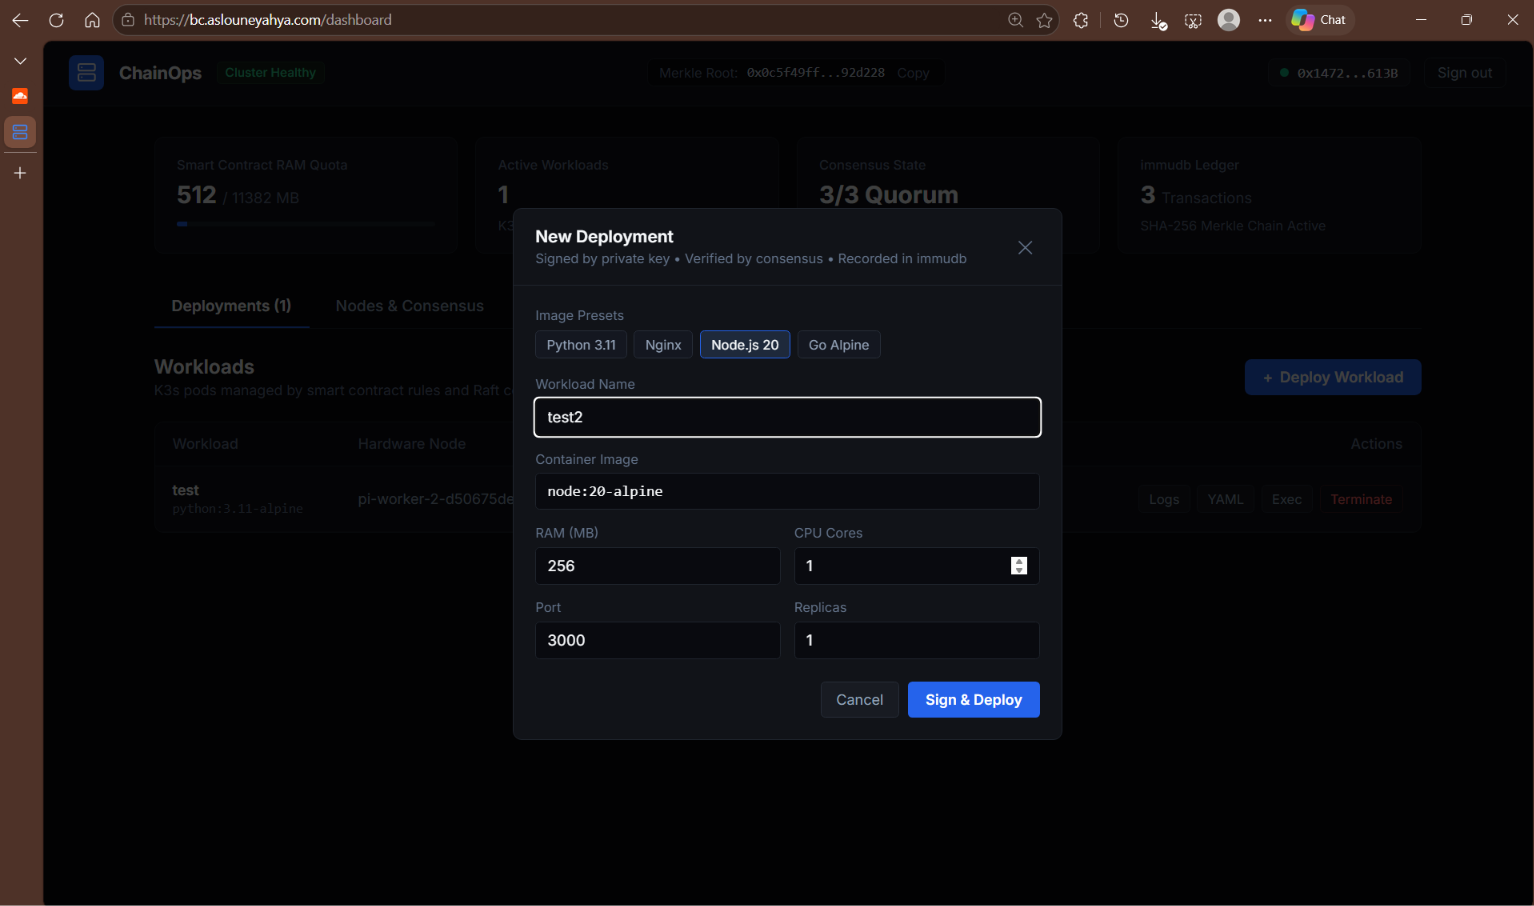
\includegraphics[width=0.82\linewidth]{figures/test2_deployment.png}
\caption{Kubernetes manifest generated by client-go alongside real-time stdout/stderr log stream}
\label{fig:test2_deployment}
\end{figure}

\subsection{Physical Node Telemetry \& Raft Quorum Health}

Figure~\ref{fig:nodes_consensus} validates bare-metal telemetry reflecting distinct hardware roles:

\begin{figure}[H]
\centering
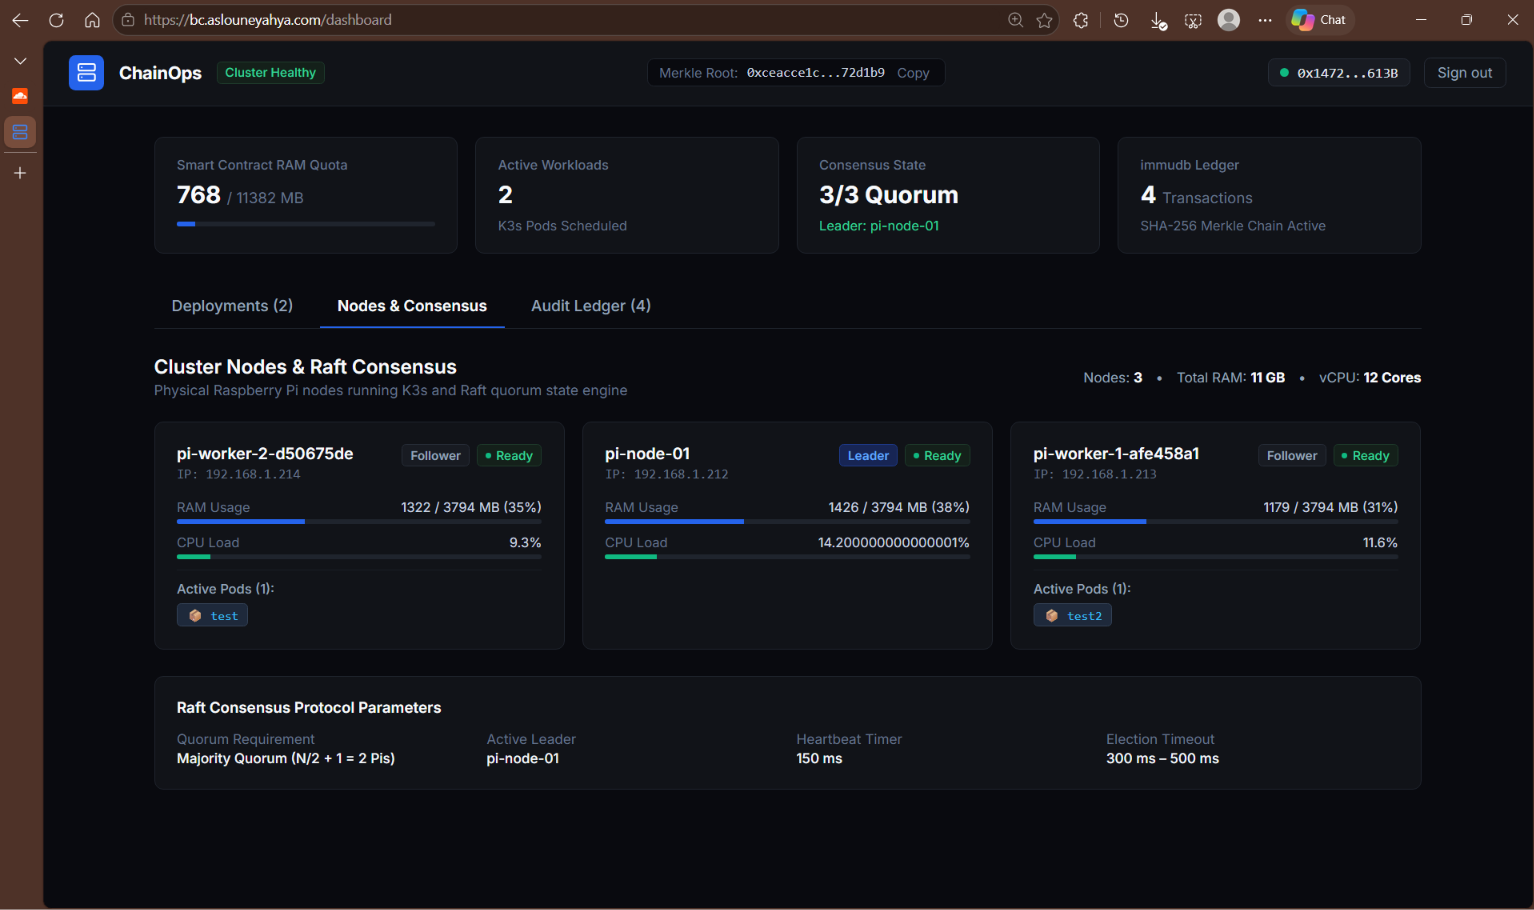
\includegraphics[width=0.82\linewidth]{figures/nodes_consensus.png}
\caption{Real-time hardware telemetry and Raft quorum voting parameters across all 3 Raspberry Pis}
\label{fig:nodes_consensus}
\end{figure}

\begin{itemize}[leftmargin=1.2cm]
    \item \textbf{pi-node-01} (Leader, 192.168.1.212): 1,410~MB RAM (K3s control plane, Go daemon, immudb);
    \item \textbf{pi-worker-1-afe458a1} (Follower, 192.168.1.213): 1,427~MB RAM, directly reflecting active container badge \texttt{test2};
    \item \textbf{pi-worker-2-d50675de} (Follower, 192.168.1.214): 810~MB RAM in nominal idle state.
\end{itemize}

\subsection{Immutable Blockchain Explorer \& Merkle Root}

Figure~\ref{fig:ledger} presents the cryptographic ledger explorer displaying transaction hashes, addresses, and Merkle proofs.

\begin{figure}[H]
\centering
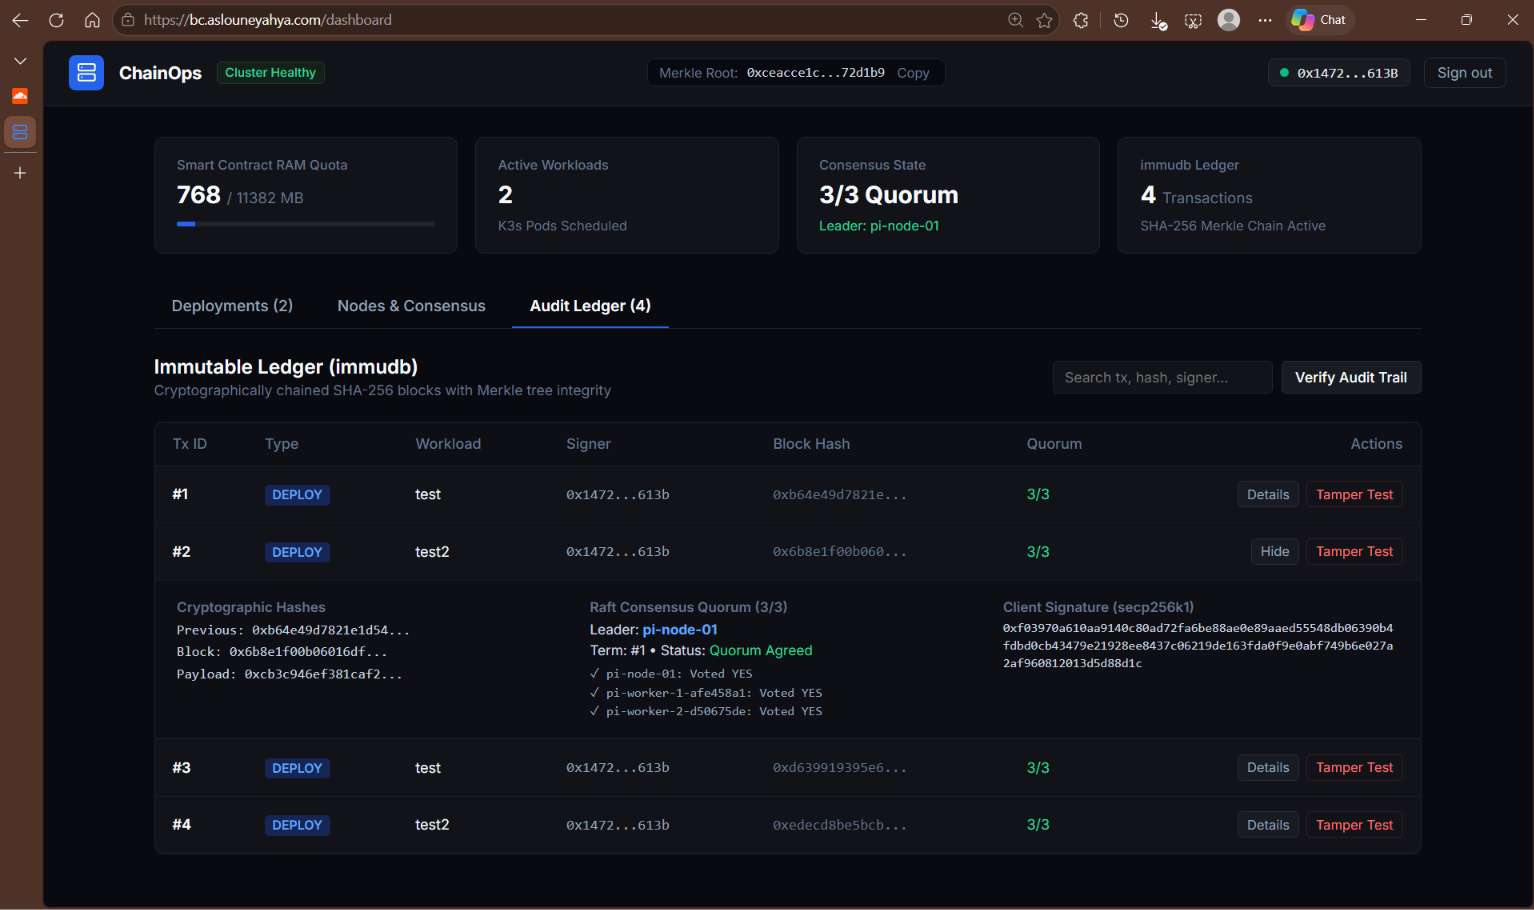
\includegraphics[width=0.82\linewidth]{figures/ledger.png}
\caption{immudb ledger explorer detailing block hashes, 3/3 Raft receipts, and Merkle root}
\label{fig:ledger}
\end{figure}

\subsection{Smart Contract Anti-OOM Quota Rejection}

Figure~\ref{fig:failed_deployment} confirms the Gatekeeper rejecting an oversized deployment exceeding the cluster's remaining physical RAM.

\begin{figure}[H]
\centering
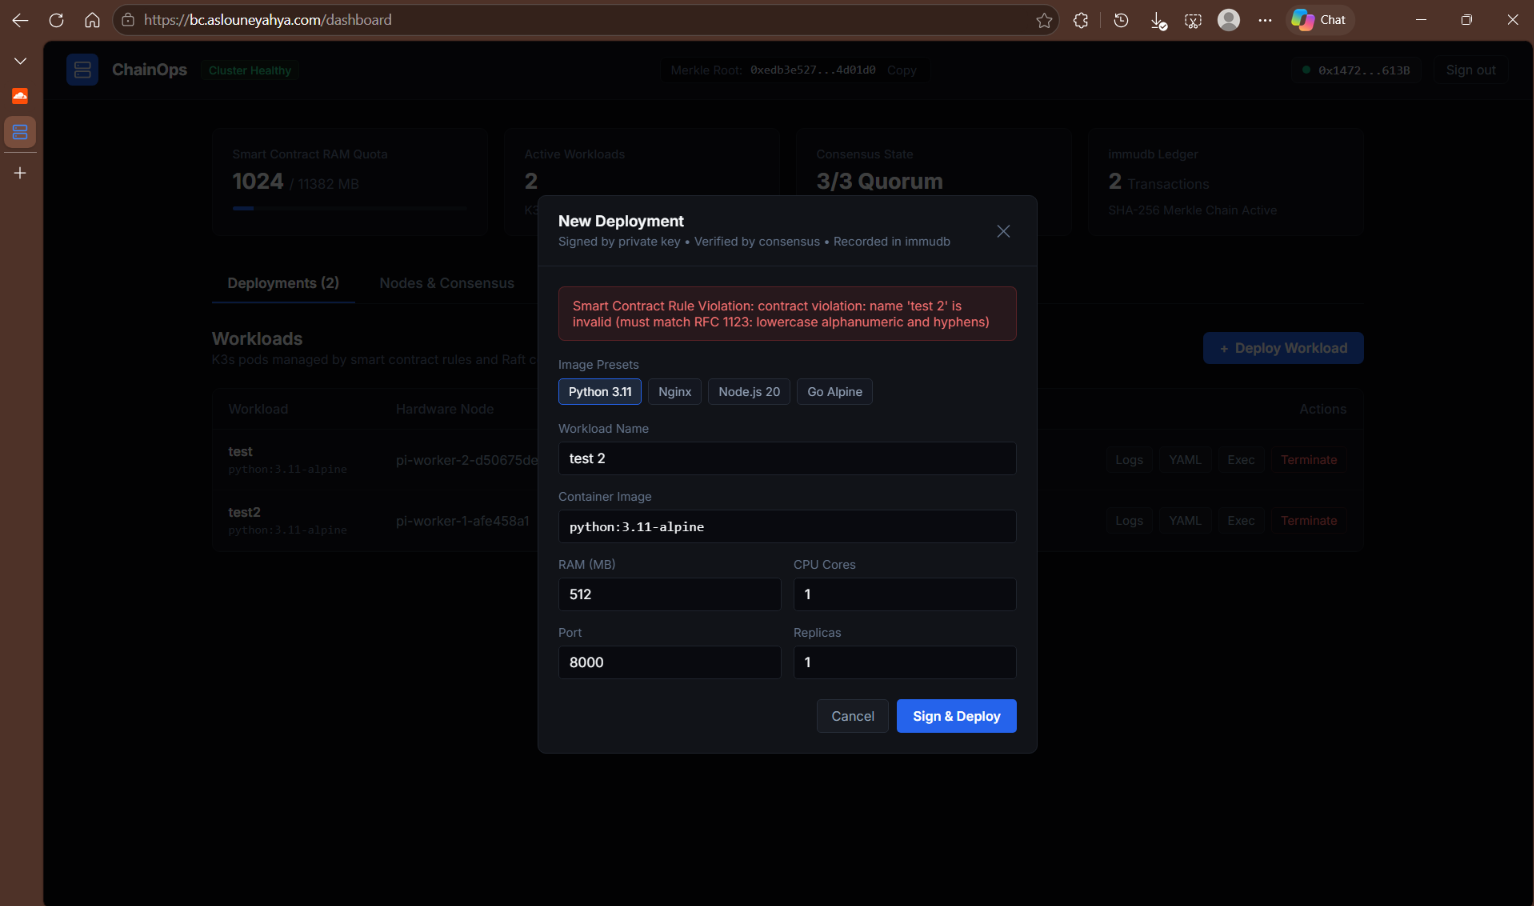
\includegraphics[width=0.82\linewidth]{figures/failed_deployment.png}
\caption{Smart Contract Gatekeeper rejecting an allocation exceeding physical bare-metal RAM capacity}
\label{fig:failed_deployment}
\end{figure}

\subsection{Physical Master Terminal Verification}

Figure~\ref{fig:raspberry_master_kubectl} shows direct monitor console output on Master Pi confirming that Kubernetes state matches the web dashboard.

\begin{figure}[H]
\centering
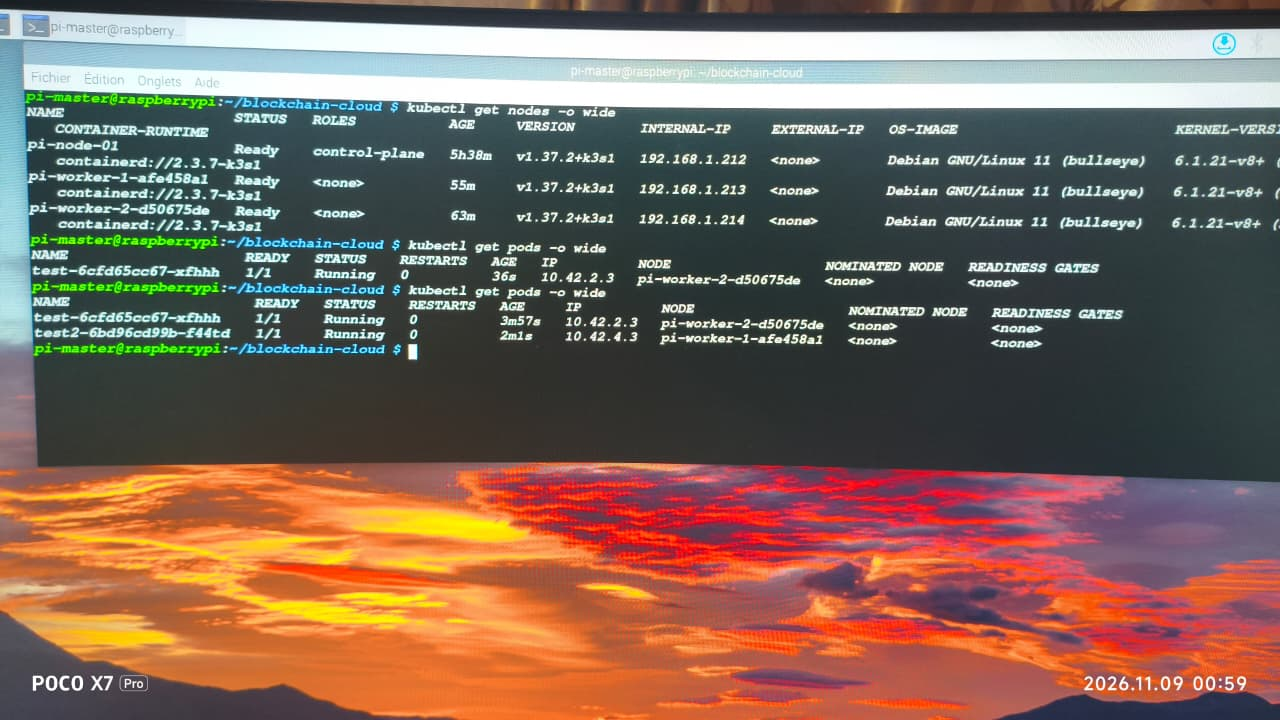
\includegraphics[width=0.82\linewidth]{figures/raspberry_master_kubectl.jpeg}
\caption{Physical Master Pi console verifying \texttt{kubectl get nodes -o wide} in Ready status}
\label{fig:raspberry_master_kubectl}
\end{figure}

\subsection{Cloudflare Zero Trust \& Local Development}

Figure~\ref{fig:infra_tools} shows the Cloudflare edge tunnel status and local Docker Compose fallback environment.

\begin{figure}[H]
\centering
\begin{subfigure}[b]{0.48\textwidth}
    \centering
    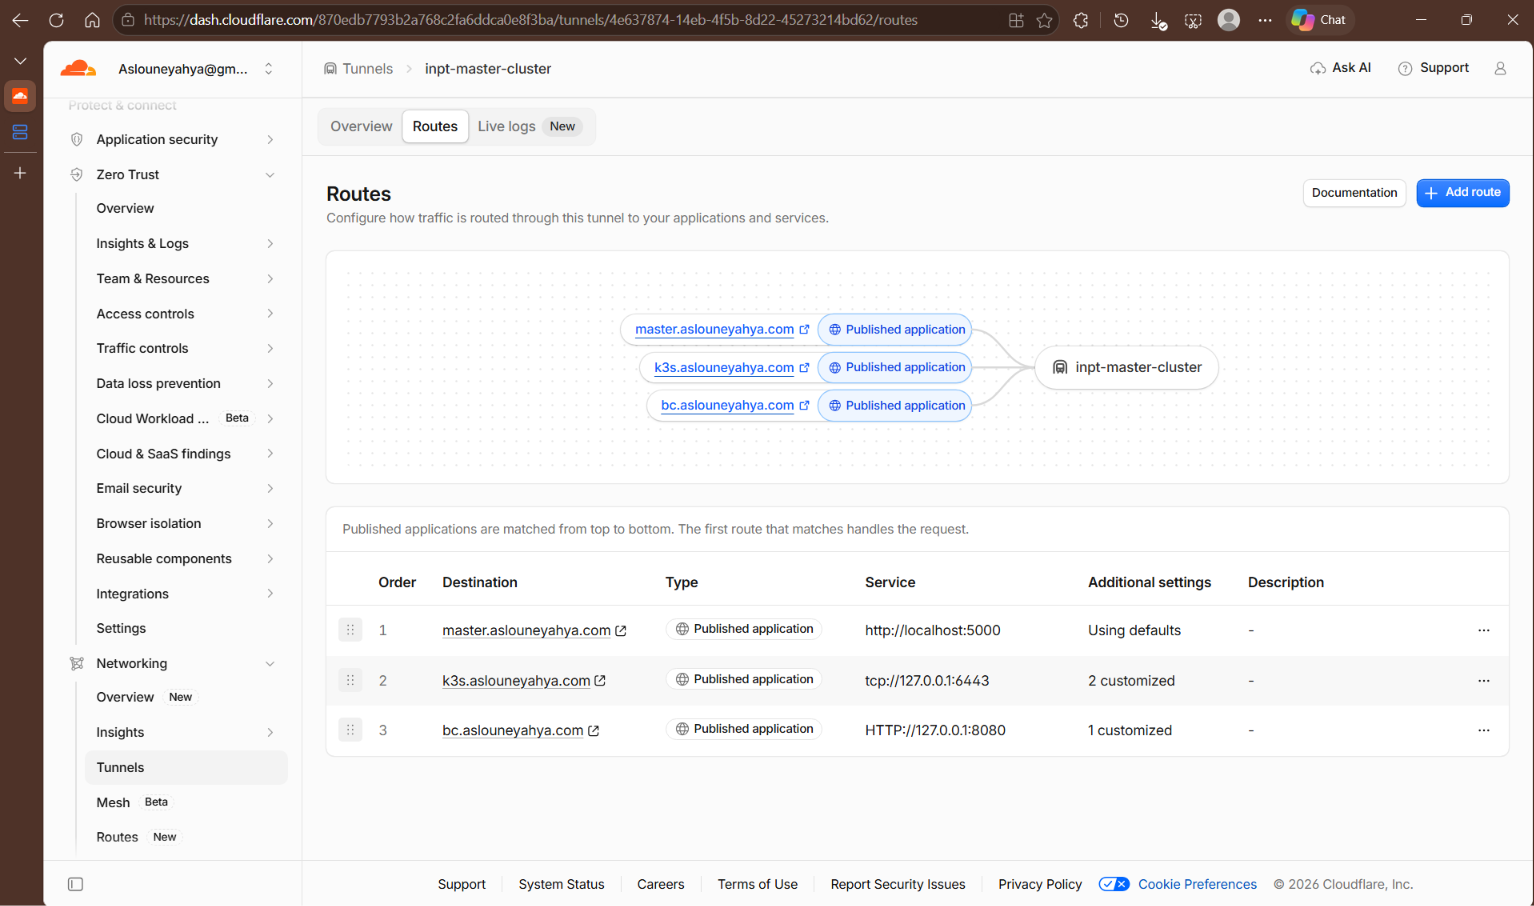
\includegraphics[width=\textwidth]{figures/cloudflare_tunnels.png}
    \caption{Cloudflare Zero Trust edge tunnels (Healthy)}
    \label{fig:cloudflare_tunnels}
\end{subfigure}
\hfill
\begin{subfigure}[b]{0.48\textwidth}
    \centering
    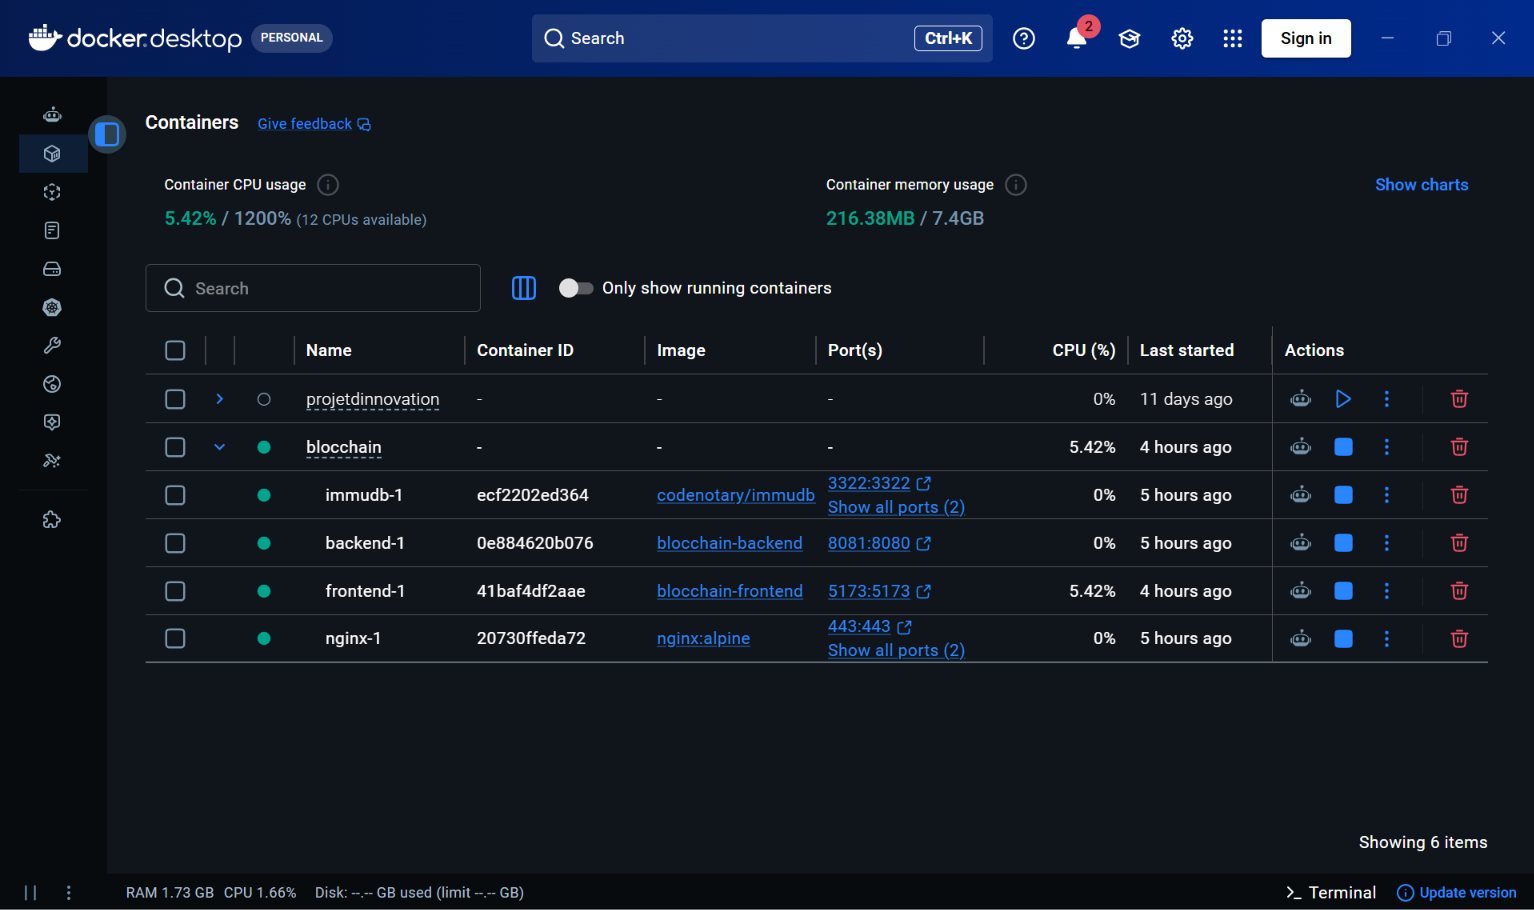
\includegraphics[width=\textwidth]{figures/local_docker.png}
    \caption{Local multi-container Docker Compose fallback}
    \label{fig:local_docker}
\end{subfigure}
\caption{Network ingress infrastructure and local development environment}
\label{fig:infra_tools}
\end{figure}

\newpage

% ==============================================================================
% SECTION 9: API SPECIFICATION & AUTOMATED CLUSTER OPERATIONS
% ==============================================================================
\section{API Specification \& Automated Cluster Operations}

\subsection{REST API Endpoint Reference}

Table~\ref{tab:api_specs} defines all REST endpoints exposed by the Go daemon at \url{https://bc.aslouneyahya.com}.

\begin{table}[H]
\centering
\footnotesize
\resizebox{\linewidth}{!}{
\begin{tabular}{|l|p{5.8cm}|p{6.2cm}|p{3.0cm}|}
\hline
\rowcolor{tableheader}
\textbf{HTTP Method} & \textbf{Endpoint Route} & \textbf{Functional Description} & \textbf{Authentication} \\
\hline
\texttt{POST} & \texttt{/api/deployments} & Executes complete 5-step consensus pipeline & $secp256k1$ Signature \\
\hline
\texttt{GET} & \texttt{/api/deployments} & Lists all live K3s deployments and pod IPs & Public \\
\hline
\texttt{GET} & \texttt{/api/deployments/\{id\}} & Retrieves full deployment specification & Public \\
\hline
\texttt{GET} & \texttt{/api/deployments/\{id\}/manifest} & Returns official generated Kubernetes YAML & Public \\
\hline
\texttt{GET} & \texttt{/api/deployments/\{id\}/logs} & Streams live stdout/stderr container logs & Public \\
\hline
\texttt{POST} & \texttt{/api/deployments/\{id\}/exec} & Executes in-pod shell commands via client-go & Public \\
\hline
\texttt{DELETE} & \texttt{/api/deployments/\{id\}} & Terminates K3s pod and commits event to immudb & $secp256k1$ Signature \\
\hline
\texttt{GET} & \texttt{/api/cluster/stats} & Global telemetry (RAM, CPU, Quorum, Leader) & Public \\
\hline
\texttt{GET} & \texttt{/api/cluster/nodes} & Hardware telemetry per physical Raspberry Pi & Public \\
\hline
\texttt{GET} & \texttt{/api/ledger} & Returns immutable transactions and Merkle root & Public \\
\hline
\texttt{GET} & \texttt{/api/ledger/audit} & Validates end-to-end cryptographic hash integrity & Public \\
\hline
\texttt{POST} & \texttt{/api/ledger/simulate-tamper} & Simulates on-disk tampering for demonstration & Public (Demo) \\
\hline
\texttt{GET} & \texttt{/api/health} & Verifies health of Raft, immudb, and K3s & Public \\
\hline
\end{tabular}
}
\caption{Complete REST API specification exposed by the unified ChainOps cluster daemon}
\label{tab:api_specs}
\end{table}

\subsection{Automated Bare-Metal Deployment}

To guarantee reproducibility, standalone zero-configuration shell scripts automate master and worker node provisioning:

\subsubsection{Master Node Deployment (Raspberry Pi 1)}
On \texttt{pi-node-01}:
\begin{lstlisting}[language=bash]
git clone https://github.com/AslouneYahya/blockchain-cloud-platform.git ~/blockchain-cloud
cd ~/blockchain-cloud
sudo bash setup_master_node.sh
\end{lstlisting}

\subsubsection{Worker Node Deployment (Raspberry Pis 2 \& 3)}
On each worker node:
\begin{lstlisting}[language=bash]
sudo bash setup_worker_node.sh pi-worker-1
sudo bash setup_worker_node.sh pi-worker-2
\end{lstlisting}
The script injects \texttt{--with-node-id} to prevent node password conflicts upon reconnecting, and establishes \texttt{k3s-tcp-tunnel.service}.

\subsubsection{Pruning Stale Inactive Nodes}
If a worker node is reinstalled, Kubernetes retains the previous registration as \texttt{NotReady}. Running the following on Master cleans the quorum immediately:
\begin{lstlisting}[language=bash]
kubectl delete node pi-worker-2
\end{lstlisting}

\newpage

% ==============================================================================
% SECTION 10: CONCLUSION & FUTURE DIRECTIONS
% ==============================================================================
\section{Conclusion \& Future Directions}

\subsection{Summary of Technical \& Academic Contributions}

Developed in the Department of Embedded Systems and Digital Services (SESNUM) at INPT under the mentorship of \textbf{Prof. Meryeme AYACHE}, this project establishes the feasibility and real-world performance of \textbf{Blockchain, Smart Contracts, and Smart Card Key Custody} applied to physical bare-metal cloud infrastructure.

Key contributions validated in production include:
\begin{itemize}[leftmargin=1.2cm]
    \item \textbf{Elimination of Centralized Trust}: Replacing session tokens with asymmetric $secp256k1$ signatures and Smart Card hardware token custody achieves non-repudiable access control;
    \item \textbf{Deterministic Hardware Admission Control}: Go-based Smart Contract enforcement mathematically prevents Out-Of-Memory kernel crashes on constrained physical nodes;
    \item \textbf{Bare-Metal Distributed Quorum}: Physical Raft consensus guarantees continuous high availability even during single-node power failures;
    \item \textbf{Provable State Immutability}: Integration with immudb Merkle trees enables sub-second detection of unauthorized manual configuration edits;
    \item \textbf{Zero-Trust Ingress Routing}: Routing mTLS over Cloudflare Layer 4 TCP bridges completely decouples nodes from local network topologies.
\end{itemize}

\subsection{Future Research Directions}

Promising research extensions include:
\begin{enumerate}[leftmargin=1.2cm]
    \item \textbf{Zero-Knowledge Workload Proofs (zk-SNARKs)}: Enabling operators to mathematically prove that a container image conforms to security compliance rules without revealing proprietary application code or environment variables;
    \item \textbf{DAO Governance}: Enforcing multi-signature ($M$-of-$N$) threshold schemes for sensitive cluster maintenance (Linux kernel upgrades, disk repartitioning);
    \item \textbf{Cryptographic State Pruning}: Developing sublinear cryptographic accumulators to prune historical blocks while preserving cryptographic audit validity on flash storage.
\end{enumerate}

\vspace{0.8cm}
\noindent\textbf{Project Repositories \& Live Platform:}
\begin{itemize}
    \item Official GitHub Repository: \url{https://github.com/AslouneYahya/blockchain-cloud-platform}
    \item INPT Institutional Repository: \url{https://github.com/AslouneYahya/cloud-platform-inpt}
    \item Live Production Platform: \url{https://bc.aslouneyahya.com}
\end{itemize}

\end{document}
